% ITY Projekt 5
% Autor: Michal Pyšík (xpysik00)

\documentclass[10pt, hyperref={unicode}]{beamer}

\usepackage[utf8]{inputenc}
\usepackage[czech]{babel}
\usepackage{times}
\usepackage{xcolor}
\usepackage{graphicx}
\usepackage{listings}
\usepackage{booktabs}

\definecolor{green_comment}{RGB}{1,63,40}
\usetheme{Copenhagen}
\beamertemplatenavigationsymbolsempty
\setbeamertemplate{footline}[frame number]
\lstset{
    extendedchars=true,
    basicstyle=\ttfamily\small,
    commentstyle=\color{green_comment},
    language=C,
    numbers=none,
	frame=single,
	keepspaces=true,
	showstringspaces=false,
	showspaces=false,
	showtabs=false,
	tabsize=4,
}
\newcommand{\centered}[1]{\begin{tabular}{l} #1 \end{tabular}}


\title{Typografie a~publikování -- 5. projekt}
\subtitle{Lineární seznam}
\author{Michal Pyšík}
\date{\today}
\institute{Vysoké učení technické v~Brně\\ Fakulta informačních technologií}





\begin{document}
\begin{frame}[noframenumbering, plain]
\maketitle
\end{frame}


\begin{frame}{Datové struktury}
\begin{itemize}
    \item Programové konstrukce sloužící k~efektivní správě dat
    \item Jsou implementací abstraktních datových typů (ADT)
    \item Definují svou vnitřní strukturu a~množinu operací, které nad nimi lze provádět
    \item Patří zde například:
        \begin{itemize}
            \item Pole
            \item Zásobník
            \item Fronta
            \item \alert{Lineární seznam}
            \item Stromové struktury
        \end{itemize}
\end{itemize}
\end{frame}


\begin{frame}{Lineární seznam}
\begin{itemize}
    \item Dynamická datová struktura
    \item Každý prvek obsahuje data a~ukazatel na další prvek
    \item Samotný seznam obsahuje pouze ukazatel na první prvek,\\
            který nazýváme hlavičkou seznamu
    \item Lineární seznam může být vázaný:
    \begin{enumerate}
        \item \alert{Jednosměrně}
        \item Obousměrně
        \item Cyklicky
    \end{enumerate}
    \item Často se navíc zavádí ukazatel na aktivní prvek seznamu
\end{itemize}
\end{frame}


\begin{frame}[fragile]{Implementace jednosměrně vázaného seznamu}
\begin{lstlisting}[title=Ukázka definice struktur v~jazyce C:]
// Struktura pro prvek seznamu
typedef struct node {
    int data; // Obsazena data
    Node *next; // Ukazatel na nasledujici prvek
} Node;

// Struktura pro samotny seznam
typedef struct list {
    Node *head; // Ukazatel na hlavicku
    Node *active; // Ukazatel na aktivni prvek
} List;
\end{lstlisting}
\end{frame}


\begin{frame}{Operace nad lineárním seznamem}
\begin{table}[]
    \centering
    \caption{Vybrané operace definované nad \alert{jednosměrně} vázaným lineárním seznamem a~jejich časová složitost 
    Omikron (nejhorší případ)}
    \begin{tabular}{ll}
        \toprule
        \textbf{Operace} & \textbf{Časová složitost} \\
        \midrule
        Hledání prvku & \quad\quad\quad $\mathcal{O}(n)$ \\
        \midrule
        Vkládání prvku & \quad\quad\quad $\mathcal{O}(n)$ \\
        \midrule
        Mazání prvku & \quad\quad\quad $\mathcal{O}(n)$ \\
        \midrule
        Reverzace seznamu & \quad\quad\quad $\mathcal{O}(n)$ \\
        \bottomrule
    \end{tabular}
    %\label{tabulka_operace}
\end{table}
\end{frame}


\begin{frame}[fragile]{Operace hledání prvku}
\begin{itemize}
    \item Sekvenčně procházíme seznamem, dokud nenalezneme hledaný prvek, nebo se nedostaneme na konec seznamu
\end{itemize}
\begin{lstlisting}[title=Hledání v~(neseřazeném) seznamu v~jazyce C:]
// funkce vraci true, pokud je hledany prvek v seznamu
bool search(Node *head, int value)
{
    Node *tmp = head;
    while(tmp != NULL)
    {
        if(tmp->data == value) return true;
        tmp = tmp->next;
    }
    return false;
}
\end{lstlisting}
\end{frame}


\begin{frame}{Operace vkládání prvku}
\begin{itemize}
    \item Rozlišujeme 3~situace:
    \begin{enumerate}
        \item Vkládání na začátek seznamu (nová hlavička)
        \item Vkládání na konec seznamu
        \item Vkládání mezi 2~prvky seznamu (nejsložitější, užitečné v~seřazených seznamech)
    \end{enumerate}
\end{itemize}
\begin{figure}[h]
    \centering
    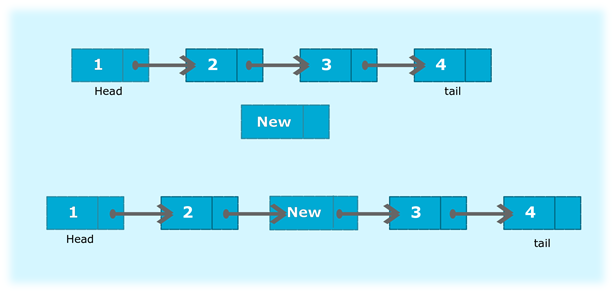
\includegraphics[scale=0.52]{insert.png}
    \caption{Vkládání nového prvku mezi 2 prvky seznamu}
\end{figure}
\end{frame}


\begin{frame}[fragile]{Operace vkládání prvku}
\begin{lstlisting}[title=Vkládání nového prvku za aktivní prvek seznamu v~jazyce C:]
void postInsert(List *L, int value)
{
    if(!Active(L)) return; // Neni nastaven aktivni prvek
    
    Node *tmp = malloc(sizeof(Node));
    if(tmp == NULL)
    {
        // Osetrit spatnou alokaci
        return;
    }
	tmp->data = value;
	tmp->next = L->active->next;
	L->active->next = tmp;
}
\end{lstlisting}
\end{frame}


\begin{frame}{Operace mazání prvku}
\begin{itemize}
    \item Opět lze rozdělit na 3 situace, analogicky ke vkládání
    \item Při smazání aktivního prvku aktivita seznamu zaniká
\end{itemize}
\begin{figure}[h]
    \centering
    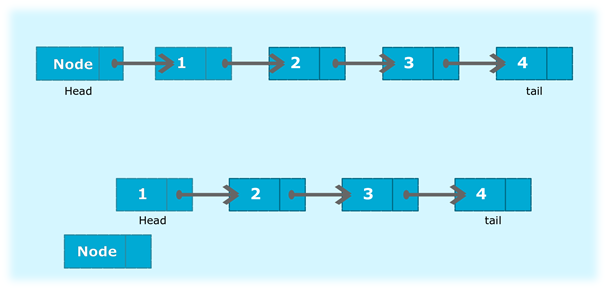
\includegraphics[scale=0.52]{delete.png}
    \caption{Mazání prvku ze začátku seznamu}
\end{figure}
\end{frame}


\begin{frame}[fragile]{Operace mazání prvku}
\begin{lstlisting}[title=Mazání prvku za aktivním prvkem seznamu v~jazyce C:]
void postDelete(List *L)
{
    if(!Active(L)) return;
    
 	Node tmp = L->active->next;
	if(tmp != NULL)
	{
		L->active->next = tmp->next;
		tmp->next = NULL;
		free(tmp);
	}
}
\end{lstlisting}
\end{frame}


\begin{frame}{Použité zdroje}
\begin{thebibliography}{}
\bibitem{} Předmět Algoritmy (IAL)
    \newblock \url{https://www.fit.vut.cz/study/course/13948/.cs}
\bibitem{} JavaTpoint
    \newblock \url{https://www.javatpoint.com/}
\end{thebibliography}
\end{frame}


\end{document}
